\documentclass[a4paper]{article}\usepackage[]{graphicx}\usepackage[]{color}
%% maxwidth is the original width if it is less than linewidth
%% otherwise use linewidth (to make sure the graphics do not exceed the margin)
\makeatletter
\def\maxwidth{ %
  \ifdim\Gin@nat@width>\linewidth
    \linewidth
  \else
    \Gin@nat@width
  \fi
}
\makeatother

\definecolor{fgcolor}{rgb}{0.345, 0.345, 0.345}
\newcommand{\hlnum}[1]{\textcolor[rgb]{0.686,0.059,0.569}{#1}}%
\newcommand{\hlstr}[1]{\textcolor[rgb]{0.192,0.494,0.8}{#1}}%
\newcommand{\hlcom}[1]{\textcolor[rgb]{0.678,0.584,0.686}{\textit{#1}}}%
\newcommand{\hlopt}[1]{\textcolor[rgb]{0,0,0}{#1}}%
\newcommand{\hlstd}[1]{\textcolor[rgb]{0.345,0.345,0.345}{#1}}%
\newcommand{\hlkwa}[1]{\textcolor[rgb]{0.161,0.373,0.58}{\textbf{#1}}}%
\newcommand{\hlkwb}[1]{\textcolor[rgb]{0.69,0.353,0.396}{#1}}%
\newcommand{\hlkwc}[1]{\textcolor[rgb]{0.333,0.667,0.333}{#1}}%
\newcommand{\hlkwd}[1]{\textcolor[rgb]{0.737,0.353,0.396}{\textbf{#1}}}%
\let\hlipl\hlkwb

\usepackage{framed}
\makeatletter
\newenvironment{kframe}{%
 \def\at@end@of@kframe{}%
 \ifinner\ifhmode%
  \def\at@end@of@kframe{\end{minipage}}%
  \begin{minipage}{\columnwidth}%
 \fi\fi%
 \def\FrameCommand##1{\hskip\@totalleftmargin \hskip-\fboxsep
 \colorbox{shadecolor}{##1}\hskip-\fboxsep
     % There is no \\@totalrightmargin, so:
     \hskip-\linewidth \hskip-\@totalleftmargin \hskip\columnwidth}%
 \MakeFramed {\advance\hsize-\width
   \@totalleftmargin\z@ \linewidth\hsize
   \@setminipage}}%
 {\par\unskip\endMakeFramed%
 \at@end@of@kframe}
\makeatother

\definecolor{shadecolor}{rgb}{.97, .97, .97}
\definecolor{messagecolor}{rgb}{0, 0, 0}
\definecolor{warningcolor}{rgb}{1, 0, 1}
\definecolor{errorcolor}{rgb}{1, 0, 0}
\newenvironment{knitrout}{}{} % an empty environment to be redefined in TeX

\usepackage{alltt}

%%% Преамбула!

\usepackage[utf8]{inputenc}
\usepackage[russian]{babel}
\usepackage[X2,T2A]{fontenc}

\usepackage[paper=a4paper,top=13.5mm, bottom=13.5mm, left=16.5mm, right=13.5mm, includefoot]{geometry}
\usepackage[unicode,colorlinks=true,urlcolor=blue,hyperindex,breaklinks]{hyperref}
\usepackage{amsmath,amsfonts,amssymb,amsthm,mathtools} 

\usepackage{indentfirst} % установка отступа в первом абзаце главы!!!

\title{Отчёт о проделанной работе}
\author{Хрюша}
\date{\today}
\IfFileExists{upquote.sty}{\usepackage{upquote}}{}
\begin{document}

\maketitle

\section{Основовы}




Тут можно писать текст, и даже вот такие вот формулы

\[ \int_{0}^{+\infty} x^{s-1} \cdot e^{-x} dx = \Gamma(s). \]

Всё совсем как в \LaTeX! Но у нас нет на это времени! Пора строить графики!



\begin{table}[h!]

\begin{tabular}{l|r|r|r|r|r|r}
\hline
t & GOOG.Open & GOOG.High & GOOG.Low & GOOG.Close & GOOG.Volume & GOOG.Adjusted\\
\hline
2016-01-04 & 743.00 & 744.060 & 731.258 & 741.84 & 3272800 & 741.84\\
\hline
2016-01-05 & 746.45 & 752.000 & 738.640 & 742.58 & 1950700 & 742.58\\
\hline
2016-01-06 & 730.00 & 747.180 & 728.920 & 743.62 & 1947000 & 743.62\\
\hline
2016-01-07 & 730.31 & 738.500 & 719.060 & 726.39 & 2963700 & 726.39\\
\hline
2016-01-08 & 731.45 & 733.230 & 713.000 & 714.47 & 2450900 & 714.47\\
\hline
2016-01-11 & 716.61 & 718.855 & 703.540 & 716.03 & 2090600 & 716.03\\
\hline
\end{tabular}


\caption{Стоимость акций}
\end{table}


Графики можно построить совсем разными. Например, вот такой! 


\begin{knitrout}
\definecolor{shadecolor}{rgb}{0.969, 0.969, 0.969}\color{fgcolor}

{\centering 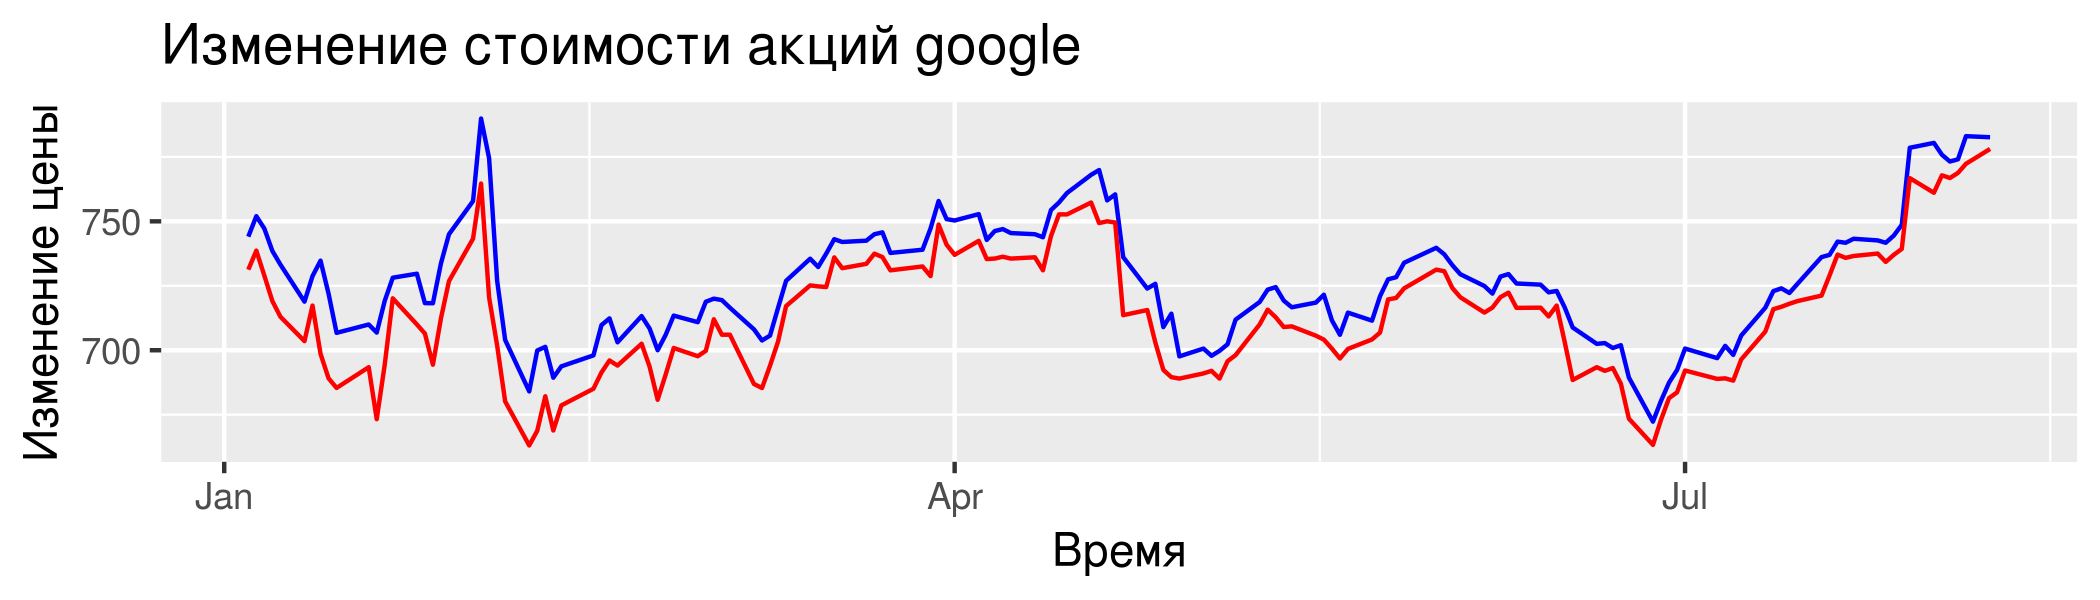
\includegraphics[width=\maxwidth]{figure/unnamed-chunk-3-1} 

}



\end{knitrout}

Можно к коду использовать любые окружения теха! Прямо как на рисунку \ref{fig}.

\begin{figure}[h!]
\begin{knitrout}
\definecolor{shadecolor}{rgb}{0.969, 0.969, 0.969}\color{fgcolor}

{\centering 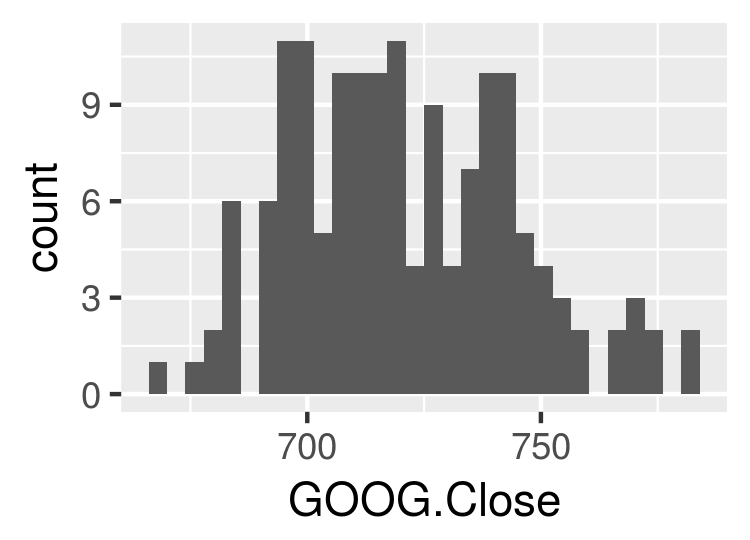
\includegraphics[width=\maxwidth]{figure/unnamed-chunk-4-1} 

}



\end{knitrout}
\caption{Гистограмка для стоимости акций гугл! \label{fig}}
\end{figure}


Средняя цена заыкрытия акции гугла рана $720.7921207$

Команда \$ \$ делает в техе формулу. Команда Sexpr обращается к R. Все, что написано в скобках к Sexpr будет посчитано в R и вставленно в \TeX. 


\section{Имена чанков}

Чанкам можно давать имена! Зачем? Например, если в коде есть ошибка, то в логах будет отражено в каком из чанков это произошло. И по имени чанка легче в большом документе найти нужный кусок. Также можно использовать эти имена в других кусках кода. Например, сделаем два чанка. При этом заблокируем в них вычисления до их вызова в следующем чанке.





Следующий чанк использует в себе информацию из чанков Вениамин и Антон! Кадый вызов - активирует созданный ранее расчёт.

\begin{knitrout}
\definecolor{shadecolor}{rgb}{0.969, 0.969, 0.969}\color{fgcolor}\begin{kframe}
\begin{verbatim}
## [1] 30
\end{verbatim}
\end{kframe}
\end{knitrout}

Такой подход к программированию не очень оптимален, так как легче написать функцию в одном из чанков, а после вызывать её выполнение в последующих. 

\end{document}
